\chapter{Circuit simulations for generating various waveform signals}
Circuit simulations were run to validate the behaviour of the conceptual design and to present the trade offs.
A harmonic balance simulation was used to investigate the concepts of chapter \ref{ch:design}, as it presented a steady state solution neglecting the transient state.
This frequency domain simulation was run with the tool \gls{ab:ads} to present the solution for the nonlinear behaviour of the test circuit.
In a first step the generation of various analog output signals were investigated.
Three basic signal waveforms were synthesized to show the ability of generating different signals.
Afterwards the designed test circuit of chapter \ref{ch:design} was tested with respect to stability and its energy consumption.
As the realized circuit differed a bit from the presented test circuit in chapter \ref{ch:design}, another simulation was run to get an impression what to expect for the measurement.
The presented simulations were run with the schematic shown in appendix \ref{app:schematic}, except for the simulation of the built demonstrator in chapter \ref{ch:ProofOfConceptWithExistingComponents}.

\section{Generating various analog signals with digital input control}
Generating analog signals from a digital input signal was the aim of the presented work.
The designed custom \gls{ab:dac}, the Riemann Pump, should be able to synthesize various waveform signals at the output.
Simulation results were presented in the time domain to validate the integrity of the desired signal.
In the system design a pre processor is used to compute the Riemann Code with a specific algorithm.
For simulation purposes the digital Riemann Code was computed manually, as seen for example in Figure \ref{fig:RiemannCodeGenerationSineWave}.
A prerequisite for the design process was a resolution of the \gls{ab:dac} of three bits.
Another prerequisite was an \gls{ab:osr} of four, as discussed in chapter \ref{ch:fundamentals}.
The presented simulations of the digital-to-analog conversion were run to proof the concept of the designed test circuit.
 
\subsection{Sine wave generation in the time domain}
As known from basic signal processing, the sine wave for continuous time is the elementary signal and therefore synthesized first. 
For the generation of this sine wave a corresponding Riemann Code was required which will be converted to the desired sine wave.\\
This Riemann Code was generated by hand via an approximation of a sine wave with a sequence of eight different slopes.
Eight different slopes represented the three bit resolution while the sequence of eight sampling points represented the \gls{ab:osr} of four. 
Figure \ref{fig:RiemannCodeGenerationSineWave} illustrates this approximation to get the corresponding Riemann Code.

%\begin{figure}[htb!]
%   \centering
%   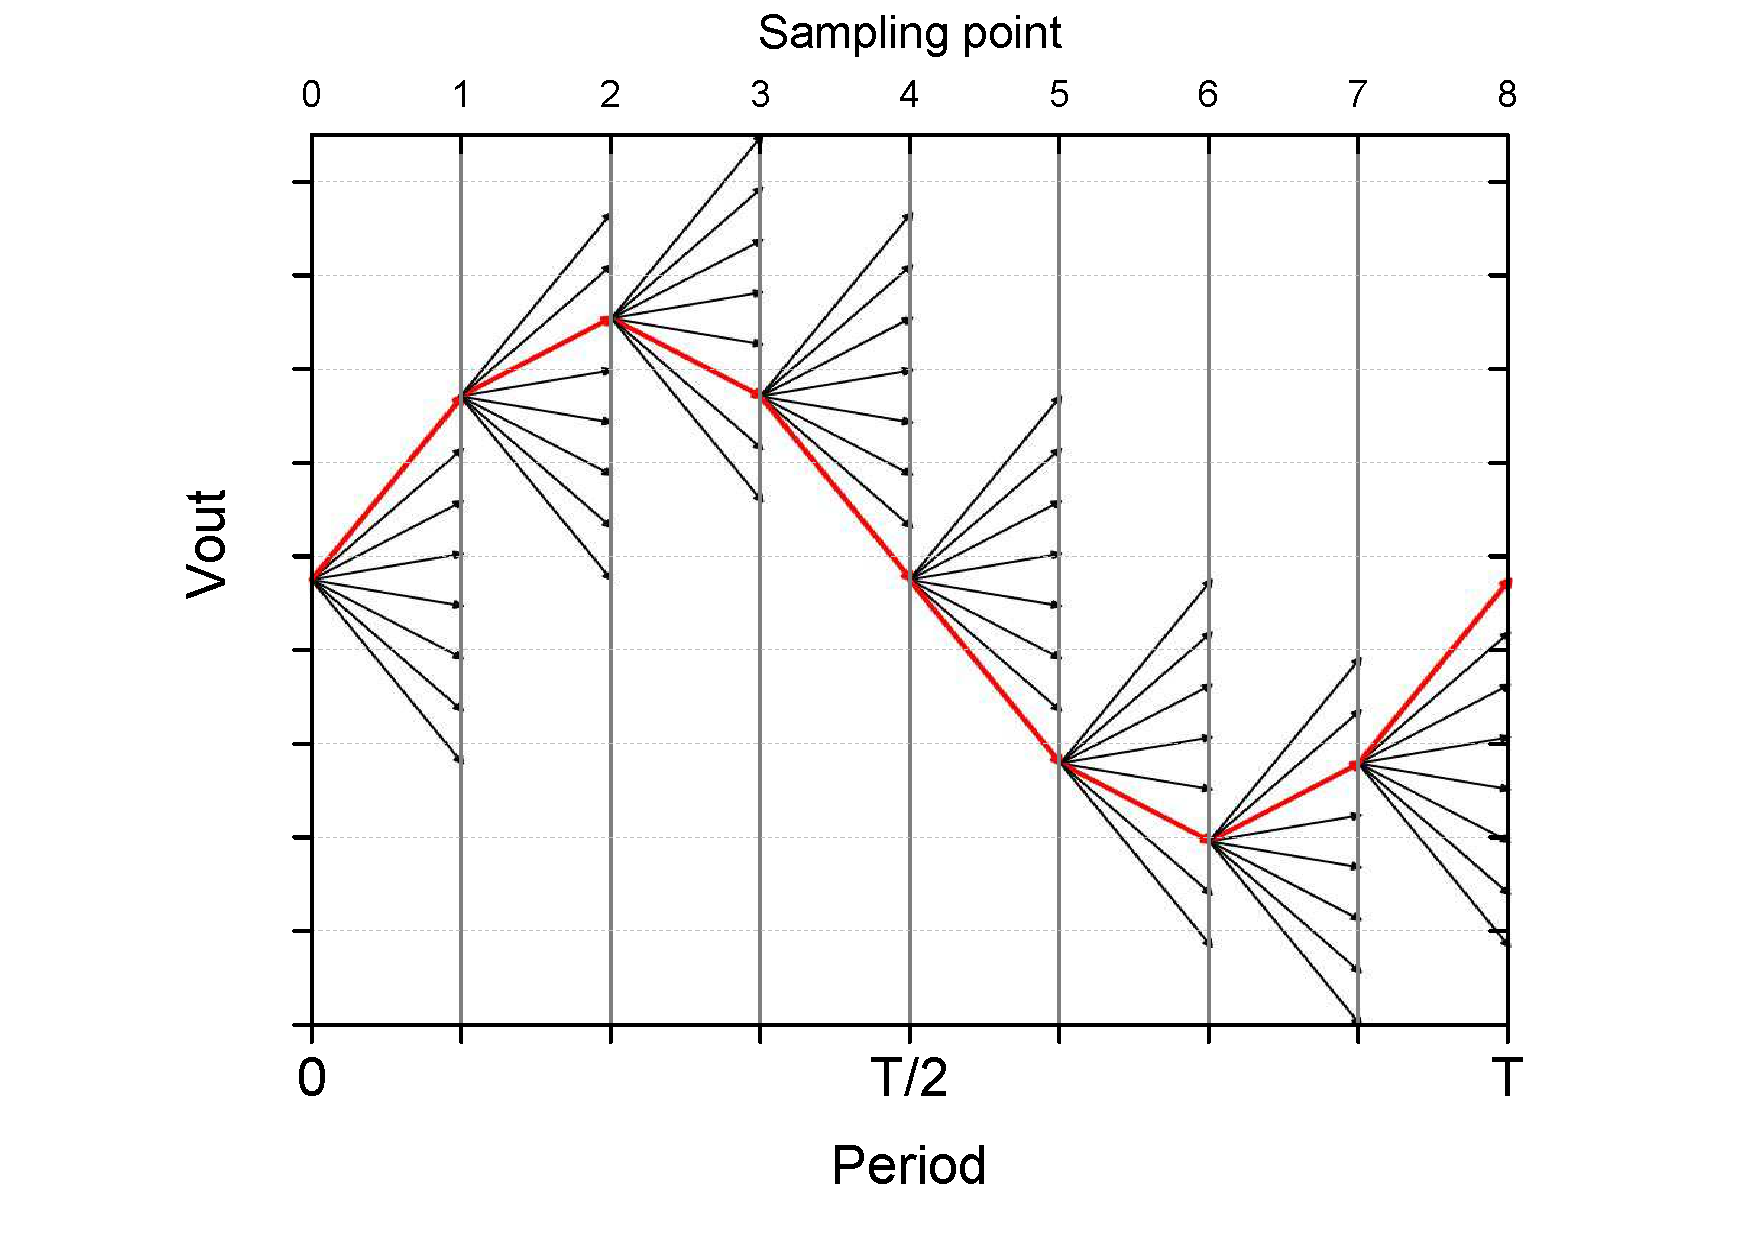
\includegraphics[width=0.75\textwidth]{RiemannCodeGeneration.pdf}
%   \caption{One possible approximation of sine wave generation to get the Riemann Code}
%   \label{fig:RiemannCodeGenerationSineWave}
%\end{figure}

%To validate the feasibility of the presented concept, a digital input control code is required.
%To get this code an approximation by hand is done since no algorithm exists which can compute this.

\begin{figure}[htb!]
   \centering 
   \input{graphics/simulation/RiemannCodeGenerationSineWave73_latest.pdf_tex}
   \caption{One possible approximation of a sine wave generation to get the Riemann Code}
   \label{fig:RiemannCodeGenerationSineWave}
\end{figure}


The sequence of chosen slopes, referred to $i_0$ values, is:
\begin{equation}
 +7\hspace{.3cm} +3\hspace{.3cm} -3\hspace{.3cm} -7\hspace{.3cm} -7\hspace{.3cm} -3\hspace{.3cm} +3\hspace{.3cm} +7,
 \end{equation} 
which represents the following encryption:
\begin{equation}
000\hspace{.3cm} 010\hspace{.3cm} 101\hspace{.3cm} 111\hspace{.3cm} 111\hspace{.3cm} 101\hspace{.3cm} 010\hspace{.3cm} 000,
\end{equation}
\label{eq:RiemannCodeSineWave} 
based on the encryption table in Figure \ref{fig:SlopesAndTable}, chapter \ref{ch:fundamentals}.
The generated Riemann Code consists of eight triplets, where each triplet represents the three bit resolution.
The quantity of digits in each set, here triplet, increases with the number of bits used for the resolution.
The number of triplets represents the number of sampling points, corresponding to the \gls{ab:osr}.
This particular generated Riemann Code in equation \ref{eq:RiemannCodeSineWave} was used to synthesize sine waves in the frequency range between \SI{500}{\MHz} and \SI{6}{\GHz}, as shown in Figure \ref{fig:7SignalsSameSlopeInOnePlot}.

\begin{figure}[htb!]
   \centering 
   \input{graphics/simulation/Vout_sine_SigBWdifferent_SameSlope_73_TwoPeriods.pdf_tex}
   \caption{Synthesized signals with demonstrated Riemann Code for the frequency range of \SI{0.5}{\GHz} to \SI{6}{\GHz}}
   \label{fig:7SignalsSameSlopeInOnePlot}
\end{figure}

The amplitude of seven signals with different frequencies are shown over their period while at the top the number of sampling points is shown.
This representation is chosen to compare the signal integrity of different frequencies.
The shape from most of the plotted functions fit fairly to a theoretical sine wave.
As the sampling interval differs for different frequencies, the amplitudes of the signals also differed.
The maximum reachable amplitude was the positive supply voltage, here set to \SI{15}{\volt}, while the lower bound was \SI{0}{\volt}. 
Once the amplitude reached the supply voltage, the signal wave form is clipped due to a fully charged output capacitor.
This undesired effect transformed the sine wave into a rectangular shaped signal form, as seen for the blue and black curve.
Therefore a bandwidth limitation is introduced.\\
Figure \ref{fig:7SignalsSameSlopeInOnePlot} highlights a limitation of the designed circuit as the blue curve turns into a rectangular signal form.\\

\begin{figure}[htb!] %% Add sampling points at the top !!
   \centering
   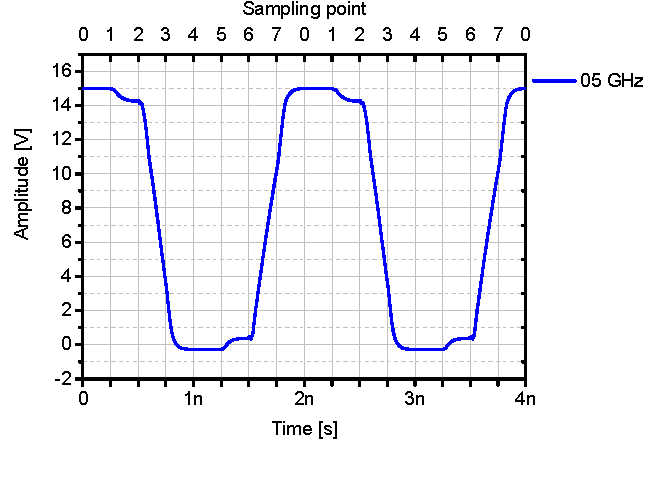
\includegraphics[width=0.75\textwidth]{Vout_sine_SigBW_05GHz_3bit_long.pdf}
   \caption{Synthesized sine wave for frequency of 0.5GHz}
   \label{fig:SineWave05GHz}
\end{figure}


Below the frequency of \SI{1}{\GHz} the desired shape of a sine wave was transformed to a rectangular  form due to the long sampling time.
In addition to the unwanted rectangular form another distortion occurred, depicted in the blue signal for the sampling interval 1 to 2 and 5 to 6.
An unsymmetrical switching process, the finite rise time of the provided current and the not perfectly defined current sources were three factors to mention. %, as the gate of the switching transistor had to be charged 
Furthermore a leakage current were induced by the commutation time of the switching process.
This distortion was mainly observed for low frequencies when the output capacitance was fully charged and discharged.
In the higher frequency range this did not effect the integrity very much.
As already mentioned in the design process, the circuit was designed to fulfil the requirement of synthesizing signals in high frequencies.\\
The signal frequency of \SI{1}{\giga \hertz} represented a lower bound on the frequency range in the used configuration. % referred to chapter \ref{ch:design} of the circuit.
The upper bound of the frequency range is limited to the detectable voltage swing of the amplitude.
If a voltage swing of \SI{2}{\volt} is still accepted, the upper bound would be a signal frequency of \SI{6}{\GHz} with the presented Riemann Code.
For lower voltage swings even higher frequencies could be reached.
In the following the signal integrity is compared in more detail.
Assuming a sine wave of the form

\begin{equation}
	v(t)= V_{DC} + \widehat{v} \cdot sin( 2  \pi  f \cdot  t + \phi),
\end{equation}
Figure \ref{fig:SineWaveSynthVsTheoretical} illustrates the comparison of this theoretical sine wave (red) with the synthesized signal (black) at frequency of \SI{1}{\GHz}.
The theoretical sine wave had an amplitude of $\widehat{v} = \SI{7.5}{\volt}$, a signal frequency of $f = \SI{1}{\giga \hertz}$, a phase shift of approximately $\phi = \pi / 4$ and an DC offset of $V_{DC} = \SI{7.5}{\volt}$.
The synthesized signal (black) is taken from Figure \ref{fig:7SignalsSameSlopeInOnePlot} and fit pretty good to the theoretical one.

\begin{figure}[htb!]
   \centering
   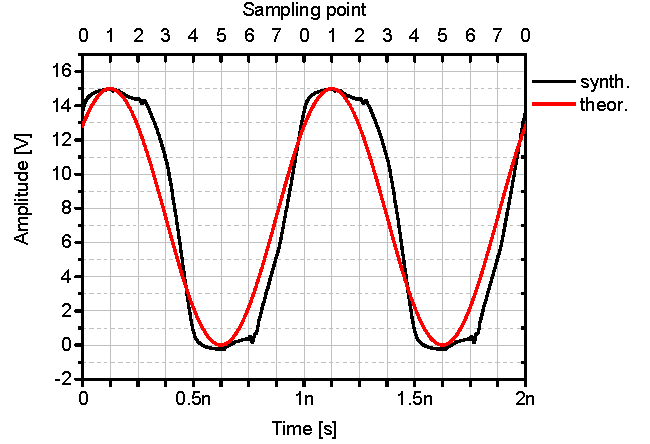
\includegraphics[width=0.75\textwidth]{Vout_SynthVsTheo.pdf}
   \caption{Synthesized sine wave with the theoretical sine wave}
   \label{fig:SineWaveSynthVsTheoretical}
\end{figure}
% 28.04.2016 19:46
Although the synthesized signal is clipped and the mentioned distortion came into play, this signal form fit relative good to the desired theoretical one.
%% 19:51 Uhr
% SQNR: 1GHz = ca. 15 dB, 2GHz = ca. 21 dB, 3GHz = 28.2 dB, 4GHz = 27.7 dB
% investigate this SNR values
Figure \ref{fig:SineCompare} highlighted the difference between the synthesized and the theoretical sine wave form in a more detailed way.

\begin{figure}[htb!]
	\centering
  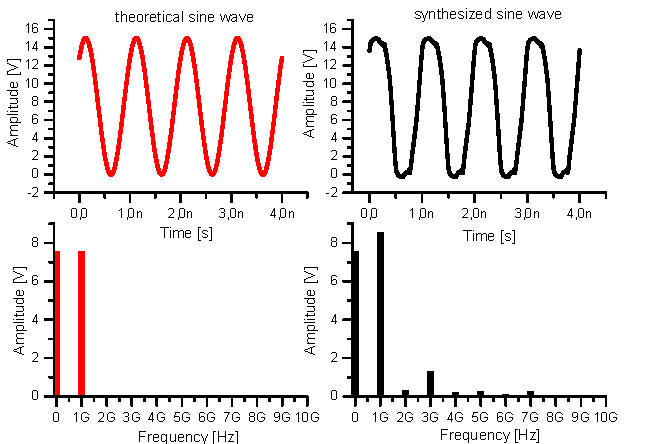
\includegraphics[width=1\textwidth]{SineCompare3.pdf}
	\caption{Comparison between a theoretical and a synthesized sine wave with their spectrum}
	\label{fig:SineCompare}
\end{figure}

A theoretical sine wave is compared to the synthesized one with their corresponding spectra.
The spectra of signals were a lot easier to compare, in contrast to the time domain signal, with respect to the accuracy.
%The spectrum of the signal demonstrates how accurate the signal is synthesized compared to a perfectly shaped sine wave. 
Since the spectrum of a perfect sine wave only consists of a DC part and the harmonic frequency it was easy to check whether the generated signal fit.\\
On the top left side of Figure \ref{fig:SineCompare} the theoretical sine wave is plotted in time domain. Underneath of it the spectrum presented a frequency portion for the direct component at \SI{0} {\Hz} and a fundamental frequency portion at \SI{1}{\GHz}.
This Fourier transformation represented the frequency portions of a clear sine wave.\\
The synthesized sine wave on the top right side fit fairly well to the theoretical one.
The spectrum of the synthesized signal showed nearly the same behaviour as for the theoretical one.
Beside the direct component and the fundamental frequency component there were some additional unwanted frequency portions which distorted the signal.
The maximum distortion was about \SI{1}{\volt} in amplitude at the third harmonic.
 The 2nd to 10th harmonic were at most half of a volt in absolute value of the amplitude.
 \textbf{The calculated \gls{ab:snr} was \SI{15.2}{\decibel}.
 The ideal \gls{ab:sqnr} of the Riemann conversion in this configuration is\SI{27}{\decibel}.}\\
% The accuracy is very good. This can be verified by the signal to noise ratio -> explain, state the SNR}
As the sampling frequency could be changed to tune the signal frequency of the output signal it was also possible to change the input control sequence to manipulate the shape of the signal.
% A limited number of different slope combinations were provided due to the restriction of the resolution.
Due to the three bit resolution there was a limited number of different slope combinations to synthesize a sine wave.
In fact the limit was bound to six different combinations for synthesizing  the sine wave, namely: 75, 73, 71, 53, 51 ,31 with respect to the $i_0$ values.
The first digit indicated the slope of the first sampling point and the second digit of the second sampling point of a rising edge from a sine wave, respectively. 
The falling edge of the sine wave consisted of the negative values of the mentioned slopes.
% A oversampling ratio of four restricted the number of combinations to six.\\

%This two slopes represent the rising edge of the sine wave and their opposite negative values the falling edge of the sine wave.
%With eight different slopes representing the full spectrum between the most negative and the most positive one, exactly four slopes can represent a rising edge of a sine wave, $+7i_0, +5i_0, +3i_0, +1i_0$.
The six different combinations were plotted in Figure \ref{fig:SameSigBWDifSlope} over two periods for the signal frequency of \SI{3}{\GHz}. 

\begin{figure}[htb!]
	\centering
  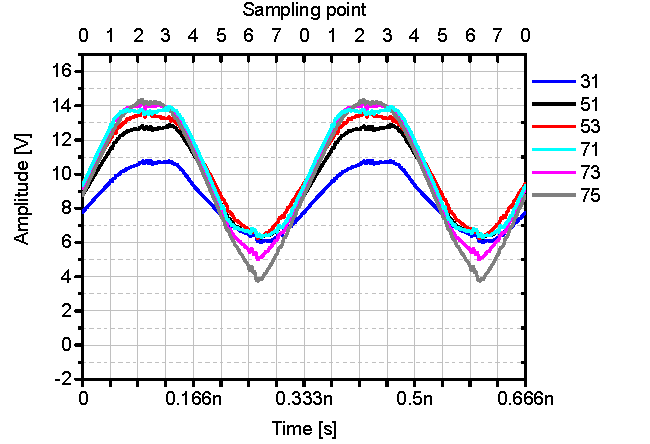
\includegraphics[width=1\textwidth]{Vout_7sine_SameSigBWdifferent_DifferentSlope.pdf}
	\caption{Signals with the same signal bandwidth \SI{3}{\giga \hertz} but different input control}
	\label{fig:SameSigBWDifSlope}
\end{figure}

Figure \ref{fig:SameSigBWDifSlope} presented the different shapes of a synthesized sine wave for a frequency of \SI{3}{\GHz}.
This was utilized to calculate the Riemann Code which fit best to the theoretical signal.


\subsection{Rectified sine wave generation in the time domain}
Beside the generation of the full sine wave, a rectified sine wave was simulated as well.\\
Based on the same approximation principle as demonstrated in figure \ref{fig:RiemannCodeGenerationSineWave}, the corresponding Riemann Code for the rectified sine was generated, namely:

%%%%%%%%%%%% this corresponds to 73 -3 -7 -7 -3 3 7
%\begin{equation}
% 000\hspace{.3cm} 010\hspace{.3cm} 101\hspace{.3cm} 111\hspace{.3cm} 000\hspace{.3cm} 010\hspace{.3cm} 101\hspace{.3cm} 111.
%\end{equation}
%\label{eq:RiemannCodeRectSine}


%% THIS CORRESPONDS TO 7 5 3 1 -1 -3 -5 -7 
%% SINCE THIS IS ENOUGH TO SYNTHESIZE A PERIOD
\begin{equation}
 000\hspace{.3cm} 001\hspace{.3cm} 010\hspace{.3cm} 011\hspace{.3cm} 100\hspace{.3cm} 101\hspace{.3cm} 110\hspace{.3cm} 111.
\end{equation}
\label{eq:RiemannCodeRectSine}

As the rectified sine wave consisted only of the positive wave form over the full period, the oversampling ratio is performed on half of a sine wave.
This resulted in a more precise wave form, since the rising and falling edges could be synthesized in more detail.
For the sine wave the rising edge resulted in two different slopes, which was doubled for the rectified sine wave.
Hence the rectified sine wave consisted of eight sampling points, while the corresponding positive half of a sine wave only consisted of four sampling points.
The rectified sine wave exhibited the sequence of all eight different slopes, from the biggest positive to the biggest negative slope.\\
A few signals with different frequencies were simulated and plotted in figure \ref{fig:DiffSigBWSameSlope}, which used this Riemann Code.

\begin{figure}[htb!]
	\centering
  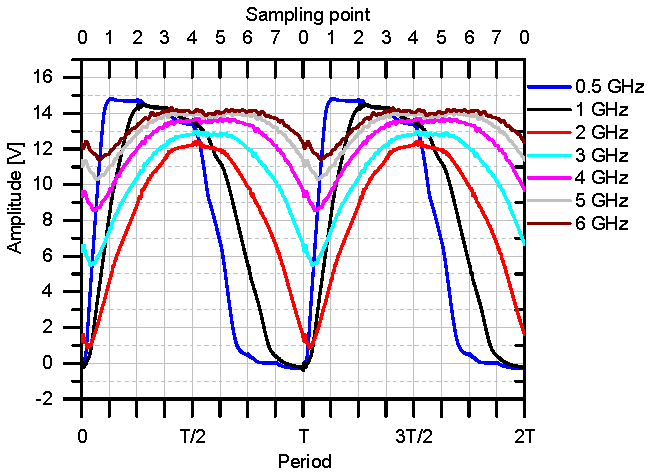
\includegraphics{Vout_halfsine_7531_diff_freq.pdf}
	\caption{Signals with same slope but different signal bandwidth}
	\label{fig:DiffSigBWSameSlope}
\end{figure}

As expected the rectified sine wave fit very good to the theoretical.
The rectified sine wave was synthesized in more detail, since the oversampling ratio were doubled effectively.
The oversampling ratio of four for the full sine wave correlated to eight sampling points for the whole period.
Since the sine wave consisted of a positive and a negative part, only four sampling points were used for the positive wave.
As the rectified sine only consisted of one positive part, eight sampling points could be used to synthesize this positive wave.
Therefore this result reflected the behaviour for a sine wave if the oversampling ratio would be doubled.
Too big absolute sampling times drove the signal into clipping for the generation of a rectified sine wave.
This effect was seen in Figure \ref{fig:DiffSigBWSameSlope} for the blue curve which had a fundamental frequency of \SI{500}{\mega \hertz}.
Since the absolute maximum voltage which could be reached was the supply voltage.
The shapes of the signals with fundamental frequencies \SI{2}{\giga \hertz} to \SI{6}{\giga \hertz} fit very good to a rectified sine, as seen in Figure \ref{fig:DiffSigBWSameSlope}.
The same issues, drawbacks and limits were presented here as for the full sine wave.
All simulations done to synthesize various signals confirmed the proof of concept.



\subsection{Triangular wave generation in the time domain}
Beside the most common signals another signal was synthesized.
A triangular signal was chosen to validate the feasibility of generating arbitrary waveforms.
The wave form of a triangular signal represented the push-pull stage charging and discharging a capacitor similarly.
As the time for charging and discharging was the same, a good fit was achieved.\\
All simulations so far were run with a three bit resolution of the realised circuit.
These three bit resolution represented eight different slopes, and therefore for a similarly charge and discharge process four different slopes could be used.
These four slopes were +7, +5, +3, +1 for the charging process and their counterparts -7, -5, -3, -1 for the discharging.
Hence the sequences of slopes were named: 11, 33, 55 and 77, with respect to $i_0$ values.
Figure \ref{fig:DiffSlopeSameBWTriangular} demonstrated the four different combinations for synthesizing the triangular wave form.

\begin{figure}[htb!]
	\centering
  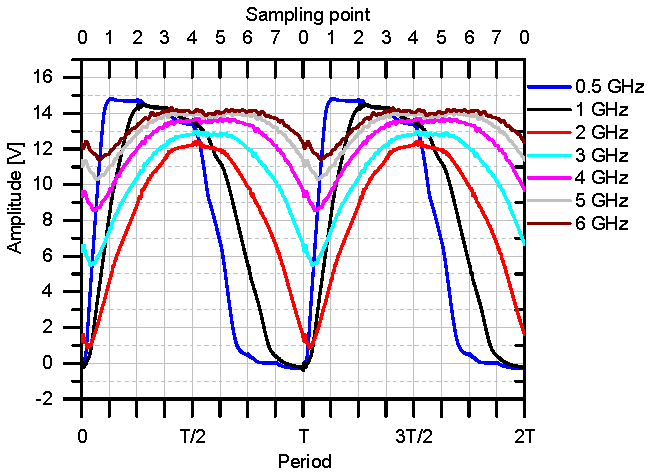
\includegraphics[draft]{Vout_halfsine_7531_diff_freq.pdf}
	\caption{Triangular signal with same signal bandwidth but different slopes}
	\label{fig:DiffSlopeSameBWTriangular}
\end{figure}

The signals were distinguished by the set of slopes used for synthesizing this shape.
The fundamental frequency was set to \SI{2}{\giga \hertz}, representative for the frequency range of \SI{500}{\mega \hertz} to \SI{6}{\giga \hertz}.
Only the wave form for the biggest slope 77 seemed to shape like a rectified sine while the other three signals seemed to fit to a triangular wave very nicely.
This effect was caused, as mentioned earlier, by the sampling time and the high current values.
This led to a clipping effect at the maximum voltage.\\
Representative for the four combinations to synthesize this triangular signal wave form, 
figure \ref{fig:DiffSigBWSameSlopeTriangular} demonstrated for the slope of 33, the frequency varying signals from \SI{500}{\mega \hertz} to \SI{6}{\giga \hertz}.


\begin{figure}[htb!]
	\centering
  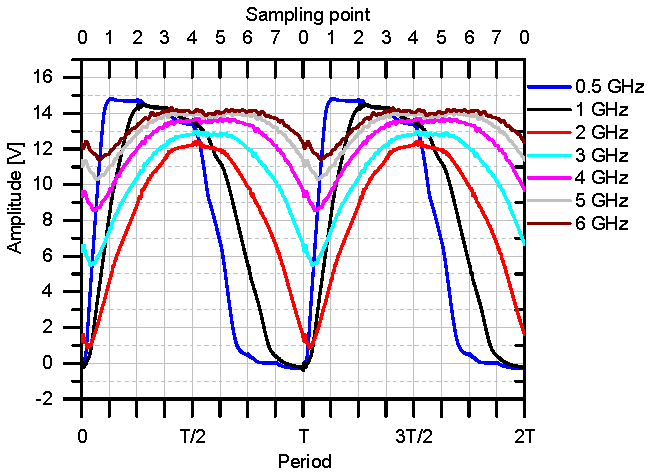
\includegraphics[draft]{Vout_halfsine_7531_diff_freq.pdf}
	\caption{Triangular signal with same slope but different signal bandwidth 3GHz}
	\label{fig:DiffSigBWSameSlopeTriangular}
\end{figure}



%The Code for the generation of the triangular signal at the output is:
%\textbf{this is not the correct code!!}
%\begin{equation}
% 000\hspace{.3cm} 010\hspace{.3cm} 101\hspace{.3cm} 111\hspace{.3cm} 000\hspace{.3cm} 010\hspace{.3cm} 101\hspace{.3cm} 111.
%\end{equation}
%\label{eq:RiemannCodeRectSine}

% short definition of stability, what cause oscillation, how to measure stability -> plot stability circles for the schematic%
\section{Stability analysis of the realised circuit}
To guarantee the proper function of the circuit a short stability analysis was performed.
This analysis was necessary to check if the circuit oscillates.
To prevent the circuit to take damage this oscillation had to be avoided.
This analysis was important to ensure that the \gls{ab:dut} was stable for the whole frequency range used.
% The analysis consisted of the measurement of S-parameters at critical points in the circuit.
 Then the complex impedance was calculated and checked if it could start an oscillation.
%The complex impedance at specific points in the circuit was measured.

To check the stability the real part of the impedance had to be positive.
A basic definition of passive elements were that they have a reflection coefficient magnitude less than unity.
Checking the input reflection coefficient, the values had to be inside the unity circle.
Therefore no negative resistance would be allowed to occur since that can lead to unwanted amplification and oscillation which can damage the circuit.
Because the real part of the impedance at all measurement points were positive for the whole frequency range, the circuit seemed to be stable.
The stability check was performed within the \gls{ab:ads} tool. 


% As switch mode power amplifier were used this was viable for the proper function of the circuit. 
\section{Energy consumption analysis of the realised circuit}
As the concept was designed for the use in mobile communication, it could be implemented in mobile devices.
Since the energy storage of mobile devices is limited, it is important to get a decent power dissipation for the whole circuit.

$ P_{cond} = R_{DS,on}dI_0^2 \propto R_{DS,on} $ \\
$ P_{sw} = \frac{1}{2} V_{in}I_0(t_{on}+t_{off})f_{sw} \propto f_{sw} $ 

In addition to the stability analysis the energy consumption analysis was important with respect to the use in mobile devices.
The losses in the circuit were those static losses while the switches plus driver is in one state.
The dynamic losses were those which occur during the switching...
Definition, expectations, simulations...

%Due to the idea to use the presented topic for mobile communication it could be implemented in mobile devices, although this thesis only handles the device for the base station. 
% If it could be used in a mobile device the energy consumption is critical.
%\\
%The energy consumption of the designed circuit in chapter \ref{ch:design} is simulated with \gls{ab:ads}.\\s
There were the trade off between the power consumption of the high side switching transistor and the switching behaviour.
Since the switching process needs to be very fast a high current is needed.
This are losses.
The driver circuit has to be optimized to reduce the energy consumption while maintaining the the switching process correctly.
If the correct hard 
\\
 For the chips used for the demonstrator refer to the work of Stephan Maroldt who states, that the power consumption is divided into static and dynamic ones. The switching losses are greater than the static ones.
% switch voltage for on/off state, switch time, static losses and dynamic losses.
In fact of the high energy consumption, the realized DAC is designed for the integration in a base station.

\section{Proof of concept simulation with existing components}
\label{ch:ProofOfConceptWithExistingComponents}
The detailed modelling and simulation of the designed circuit under real conditions, considering all loss effects would go beyond the scope of this thesis. Therefore a keep it small and simple approach was chosen.\\   
Although the used chips for the demonstrator were designed in a former work, no simulation files were available which made a detailed simulation difficult.
In the last step a simulation was run which made the concept comparable to the realized circuit. 
In this simulation the transistor dimensions were adapted to the dimension of the built demonstrator. 
This should give an insight to the behaviour of the constructed demonstrator.\\
Schematic of the measurement setup, esb.
Simulation regarding the measurement, +3 and +1 triangular waveform.
frequency 100mhz and 150mhz, vdd = 5, vdp=0V, vdn=-5V.
As DDRi2C is used, bottom vdp(in na; lowside) = vdd. 
Sim RP\_DDRi\_XY6\_v1\_sim
To combine the measurement results with the presented theory, some simulations were done with the dimensions of the real demonstrator.
%But also here it is important to note, that losses are not considered in the simulation.
It provided a basis of what can be expected.
Therefore the simulation was adapted to a two bit resolution with much greater power transistors.
To compare the results simulated here and measured in chapter \ref{ch:measurement} the switching frequencies was kept at lower frequencies (\SI{100}{\mega \hertz}).

%  This simulation should give an insight to what is expected for the measurements.
%Other important parameters to keep in mind with this simulation are the oversampling ratio and hence the switching frequency of the transistors.

 


\section{Evaluation of the simulation results for the Riemann Pump}

\begin{enumerate}
	\item different wave forms can be synthesized
	\item the signal bandwidth is restricted to a smaller one than desired
	\item parasitic effects and losses degrade the signals waveform
	\item the system is stable
	\item the energy consumption is in the range for base stations
	\item dut is not optimal w.r.t. efficiency
\end{enumerate}

%Since the digital to analog conversion always introduces noise to the signal, refer to chapter \ref{ch:fundamentals}, the fit was not perfect. 

% to increase this upper bound the transistor dimension have to be bigger
%This lower bound could be shifted to even lower frequencies if the dimensions are tuned to be smaller

% The signal frequency of \SI{1}{\giga \hertz} represented a lower bound on the frequency range in the used configuration. % referred to chapter \ref{ch:design} of the circuit.
% The upper bound of the frequency range is limited to the detectable voltage swing of the amplitude.

% implemented driver circuit which absorbed unexpected leakage currents.

%\textbf{bandwidth limitation}
%\textit{The lower bound is determined by the sampling time (inverse of the sampling frequency) and the smallest current achieved with the dimensioned transistors.
% The smallest achievable current times the smallest sampling time (highest sampling frequency) determine the smallest absolute slope achievable. \\

%The stability check was needed to validate that the circuit did not oscillate.
%As well the circuits energy consumption had to be checked, since it could be implemented in mobile devices.
% if it is in a moderate range (\textit{which is the moderate range? mention it here?}) since it could be implemented in mobile devices.\\

%If the \gls{ab:osr} is increased, the sampling time is decreased and therefore the signal quality is better because we have a more accurate synthesized signal. 
%This is shown in the snr in chapter fundamentals.

%% If the \gls{ab:osr} is increased to get a better accuracy, the switching frequency is also increased and therefore the energy consumption.
%In addition to the power consumption issue, the components have a unity current gain frequency limit.
%If the resolution is increased to get a better accuracy, the whole circuit would become more complex and the energy consumption would increase.\\
%Using the \gls{ab:osr} of four, we already get a sampling frequency of \SI{2}{GHz} at the lower bound.
%For this reason the switches have to switch within \SI{0.5}{\nano \second} which increase the gate drive current which increase the power loss.\\


% This is the trade off between the shift of the bandwidth (shifting to even higher frequencies is possible but the bandwidth is nearly constant as long the output capacitance is constant too.)  %% higher frequency means much lower sampling time which means the slopes are not detectable ... %%

%The drawback for the bandwidth shift to higher frequencies is, that with the signal frequency the switching frequency is increasing linearly (for an osr; eight times) and therefore the dynamic losses are increasing with this switching frequency.

The simulation results confirmed the feasibility of the chosen approach.
Some trade-offs in mind and the ability to change some system parameter made it possible to generate some good fitted signal waveforms.

%What is the expectation to the measurement? 
%The simulated signals with the realized dimensions of the components.
